\documentclass[12pt]{beamer}
\usetheme{LSU}
%\hypersetup{pdfpagemode=FullScreen}

\setbeamertemplate{footline}[text line]{} % makes the footer EMPTY
\useoutertheme[subsection=false]{smoothbars}

\usepackage{subfigure}
\usepackage{multicol}
\usepackage{graphicx}
\usepackage[all,knot]{xy}
\usepackage{url}
\usepackage{multimedia}
\usepackage{hyperref}
\usepackage{xcolor}
\usepackage{tabularx}

\usefonttheme{professionalfonts}
\usefonttheme{serif}
\usepackage{fontspec}
% \setmainfont{Ubuntu}
\setmainfont{Times New Roman}


\title{\Large What is ecology?}
\author{LSU -- Biol 4253}
\date{}





\begin{document}

\maketitle




% Go over syllabus, expectations, course project, grading, textbook, etc.




















%%%%% structure of lecture:

% What is ecology? --study of species interactions (intraspecific interactions, interspecific interactions, interactions with abiotic environment, etc.)


\begin{frame}

	\begin{flushright}
	  \Large \textcolor{boss2}{Ecology} 
	\end{flushright}

The study of interactions between biological organisms and their environment


\end{frame}






% Edit with pretty pictures to elaborate on each one of these.

\begin{frame}

	\begin{flushright}
	  {\Large \textcolor{boss2}{Species interactions!}}
	\end{flushright}

  With other species:

  \begin{itemize}
    \item Competition
    \item Predator -- prey
    \item Plant -- pollinator
    \item Host -- parasite
  \end{itemize}  

\end{frame}




\begin{frame}

	\begin{flushright}
	  {\Large \textcolor{boss2}{Species interactions!}}
	\end{flushright}

  With the environment:

  \begin{itemize}
    \item Abiotic variables
    \item Dispersal limitation
    \item Ecosystem respiration 
    \item Ecosystem engineering
  \end{itemize}  
\end{frame}
















% What isn't ecology?



\begin{frame}

  {\Large  \textcolor{boss1}{What is not ecology?}} \\

\end{frame}





%Discuss these individually. What do they share in common, and how do they fundamentally differ?

\begin{frame}

	\begin{flushright}
	  \Large \textcolor{boss2}{Environmentalism} \\
	  \Large \textcolor{boss3}{Biomedicine} \\
	  \Large \textcolor{boss4}{Natural history} \\
	  \Large \textcolor{boss5}{Evolution} \\
	\end{flushright}
\end{frame}










% Levels of biological organization (individual, population, community, ecosystem)--drill down into each one of these.


\begin{frame}

  \textcolor{boss5}{Levels of biological organization}\\
  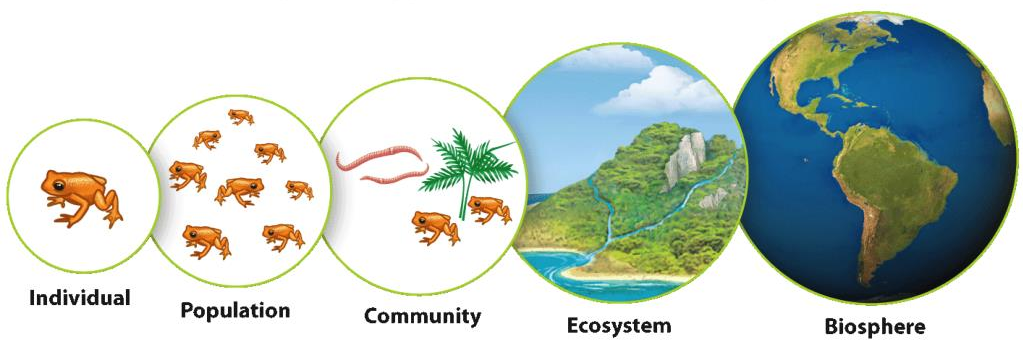
\includegraphics[width=\textwidth]{figs/ecologicalOrganization.png}
\end{frame}



\begin{frame}

	\begin{flushright}
	  \Large \textcolor{boss2}{Individual} 
	\end{flushright}

A single individual of a species.  \\

e.g., a single trout in lake superior
\end{frame}







\begin{frame}

	\begin{flushright}
	  \Large \textcolor{boss2}{Population} 
	\end{flushright}

A collection of individuals that occupy a given geographic area and interact with one another.\\

e.g., trout in lake superior
\end{frame}









\begin{frame}

	\begin{flushright}
	  \Large \textcolor{boss2}{Community} 
	\end{flushright}

A set of interacting species that occupy a given geographic area.\\

e.g., fish communities in lake superior
\end{frame}











\begin{frame}

	\begin{flushright}
	  \Large \textcolor{boss2}{Ecosystem} 
	\end{flushright}
The set of interacting species (the community) and the interactions between these species and their physical environment. \\

e.g., lake
\end{frame}











\begin{frame}

	\begin{flushright}
	  \Large \textcolor{boss2}{Biosphere} 
	\end{flushright}

The global environment, consisting of all living things on the planet.

e.g., the planet

\end{frame}




























% What is the role of the environment and land use change to each level?


\begin{frame}

	\begin{flushright}
	  \Large \textcolor{boss2}{Individual} 
	\end{flushright}

  \begin{center}
    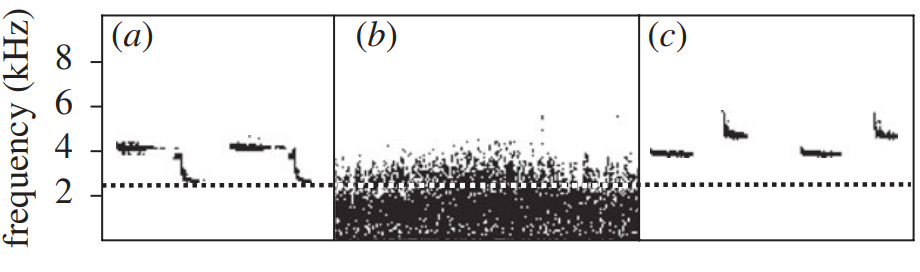
\includegraphics[width=\textwidth]{figs/individual.png}
  \end{center}
  \let\thefootnote\relax\footnotetext{Mockford and Marshall 2009 \textit{Proceedings B}}

\end{frame}












\begin{frame}

	\begin{flushright}
	  \Large \textcolor{boss2}{Population} 
	\end{flushright}
%  Fertilizer, habitat loss, introduced species, pollution all influence population size.
%  Population dynamics may be driven by environment.\\
%  More variable environments result in increased extinction risk (climate change increases environmental variability) \\

  \begin{center}
    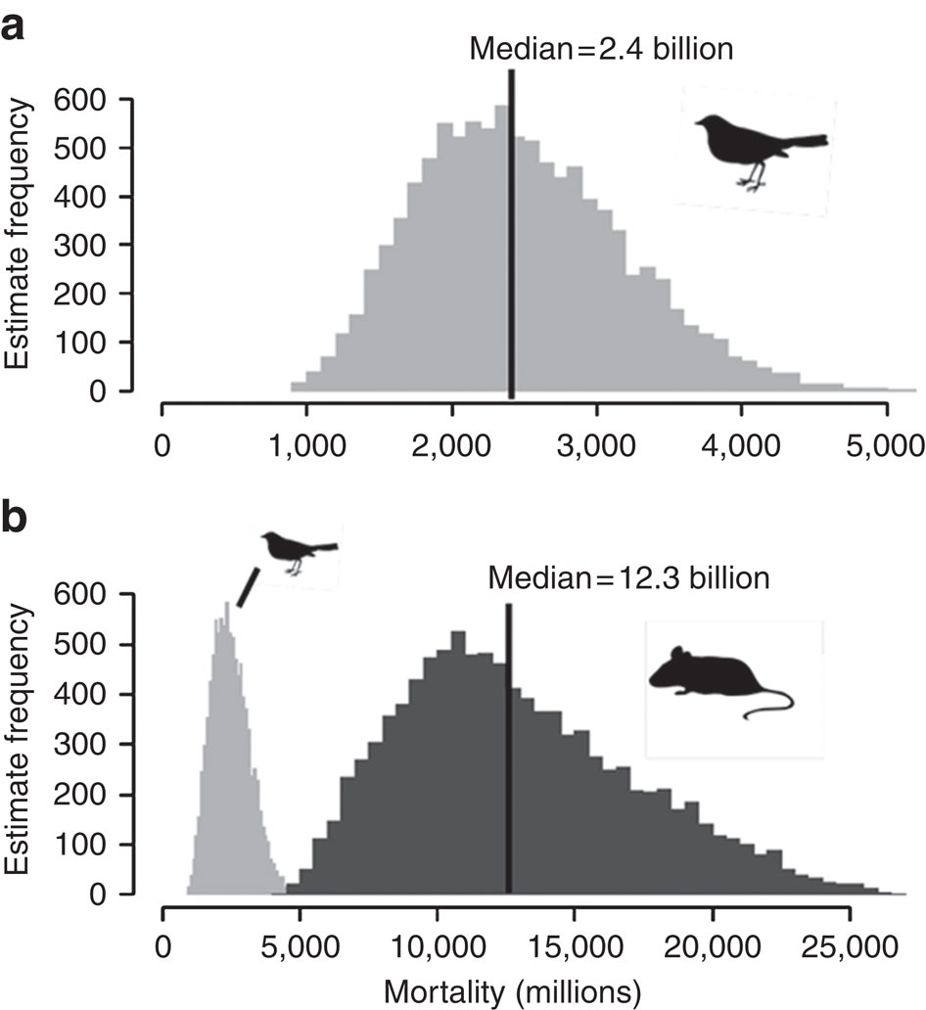
\includegraphics[width=0.6\textwidth]{figs/population.jpg}
  \end{center}
  \let\thefootnote\relax\footnotetext{Loss, Will, and Marra 2013 \textit{Nature Communications}}

\end{frame}








\begin{frame}

	\begin{flushright}
	  \Large \textcolor{boss2}{Community} 
	\end{flushright}
  
%  Fertilizer, habitat loss, introduced species, pollution affect individual species, but also influence interactions among community members (e.g., shared prey). 
  \begin{center}
    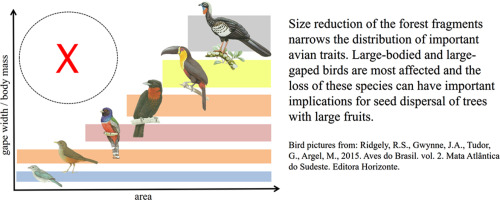
\includegraphics[width=\textwidth]{figs/community.jpg}
  \end{center}
  \let\thefootnote\relax\footnotetext{Bovo et al. 2018 \textit{Perspectives in Ecology and Conservation}}
\end{frame}







\begin{frame}

	\begin{flushright}
	  \Large \textcolor{boss2}{Ecosystem} 
	\end{flushright}

%Fertilizer, habitat loss, introduced species, pollution affect ecosystems (e.g., eutrophication) 
  \begin{center}
    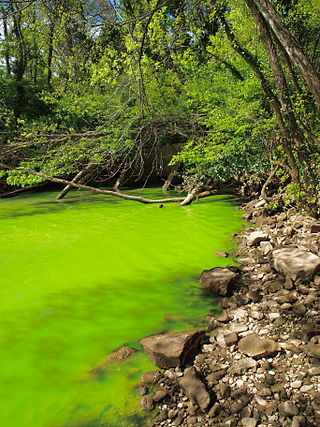
\includegraphics[width=0.45\textwidth]{figs/ecosystem.jpg}
  \end{center}
  \let\thefootnote\relax\footnotetext{Alexandr Trubetskoy}
\end{frame}






\begin{frame}

	\begin{flushright}
	  \Large \textcolor{boss2}{Biosphere} 
	\end{flushright}

%Fertilizer, habitat loss, introduced species, pollution affect large-scale patterns of diversity (e.g., 
  \begin{center}
    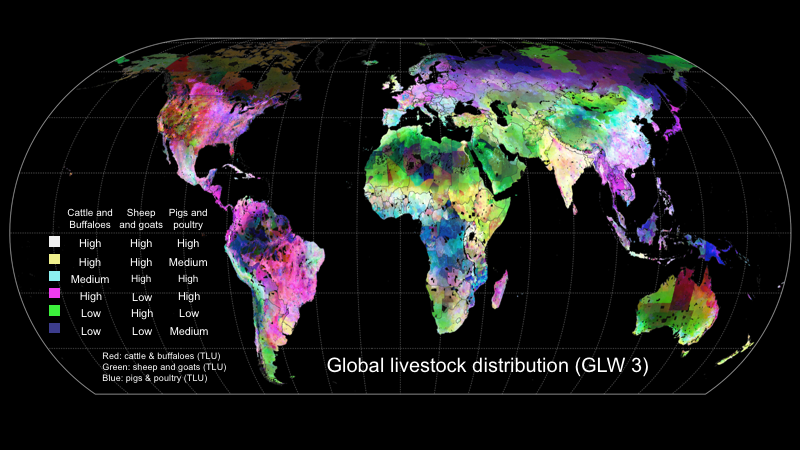
\includegraphics[width=\textwidth]{figs/globalRisk.png}
  \end{center}
  \let\thefootnote\relax\footnotetext{Gilbert et al. 2018 \textit{Nature Scientific Data}}

\end{frame}


















\begin{frame}

  {\Large  \textcolor{boss1}{ How do we do ecology?}} \\

\end{frame}







\begin{frame}

	\begin{flushright}
	  \Large \textcolor{boss2}{Observations} 
	\end{flushright}


% Good way to understand species interactions (to see them).
  \begin{center}
    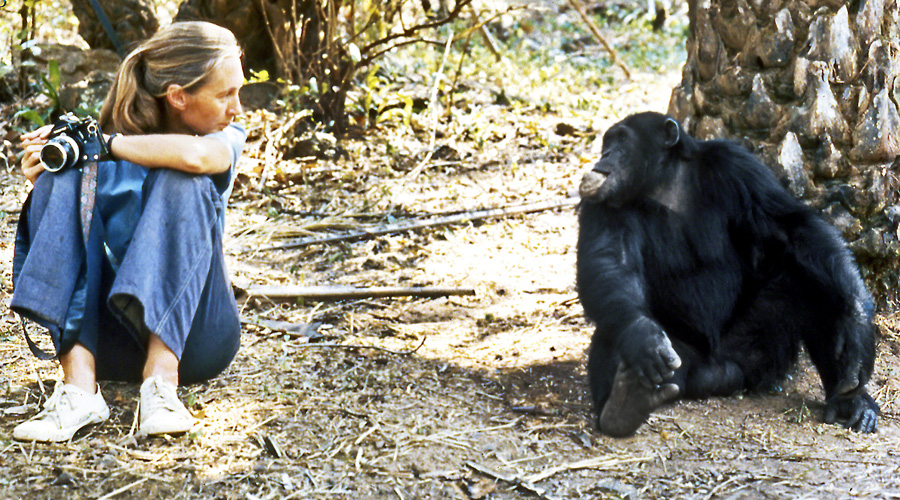
\includegraphics[width=0.95\textwidth]{figs/observation.jpg}
  \end{center}
  \let\thefootnote\relax\footnotetext{https://businesschicks.com/dr-jane-goodall-interview/}
\end{frame}





\begin{frame}

	\begin{flushright}
	  \Large \textcolor{boss2}{Field experiments} 
	\end{flushright}

%  Allows researcher to test one effect while allowing natural variability
  \begin{center}
    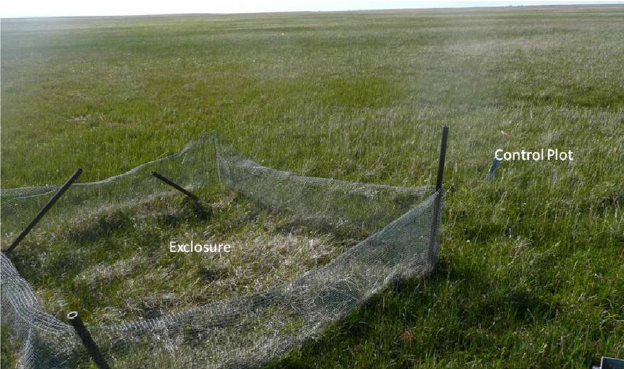
\includegraphics[width=0.95\textwidth]{figs/field.png}
  \end{center}
  \let\thefootnote\relax\footnotetext{Mark J. Lara}

\end{frame}




\begin{frame}

	\begin{flushright}
	  \Large \textcolor{boss2}{Laboratory experiments} 
	\end{flushright}
%  Allows researcher to test one (or multiple) effects while controlling variability.
%  Good for pushing system past where it might go, or for ethically questionable experiments (dose-response, pollution, etc.)
  \begin{center}
    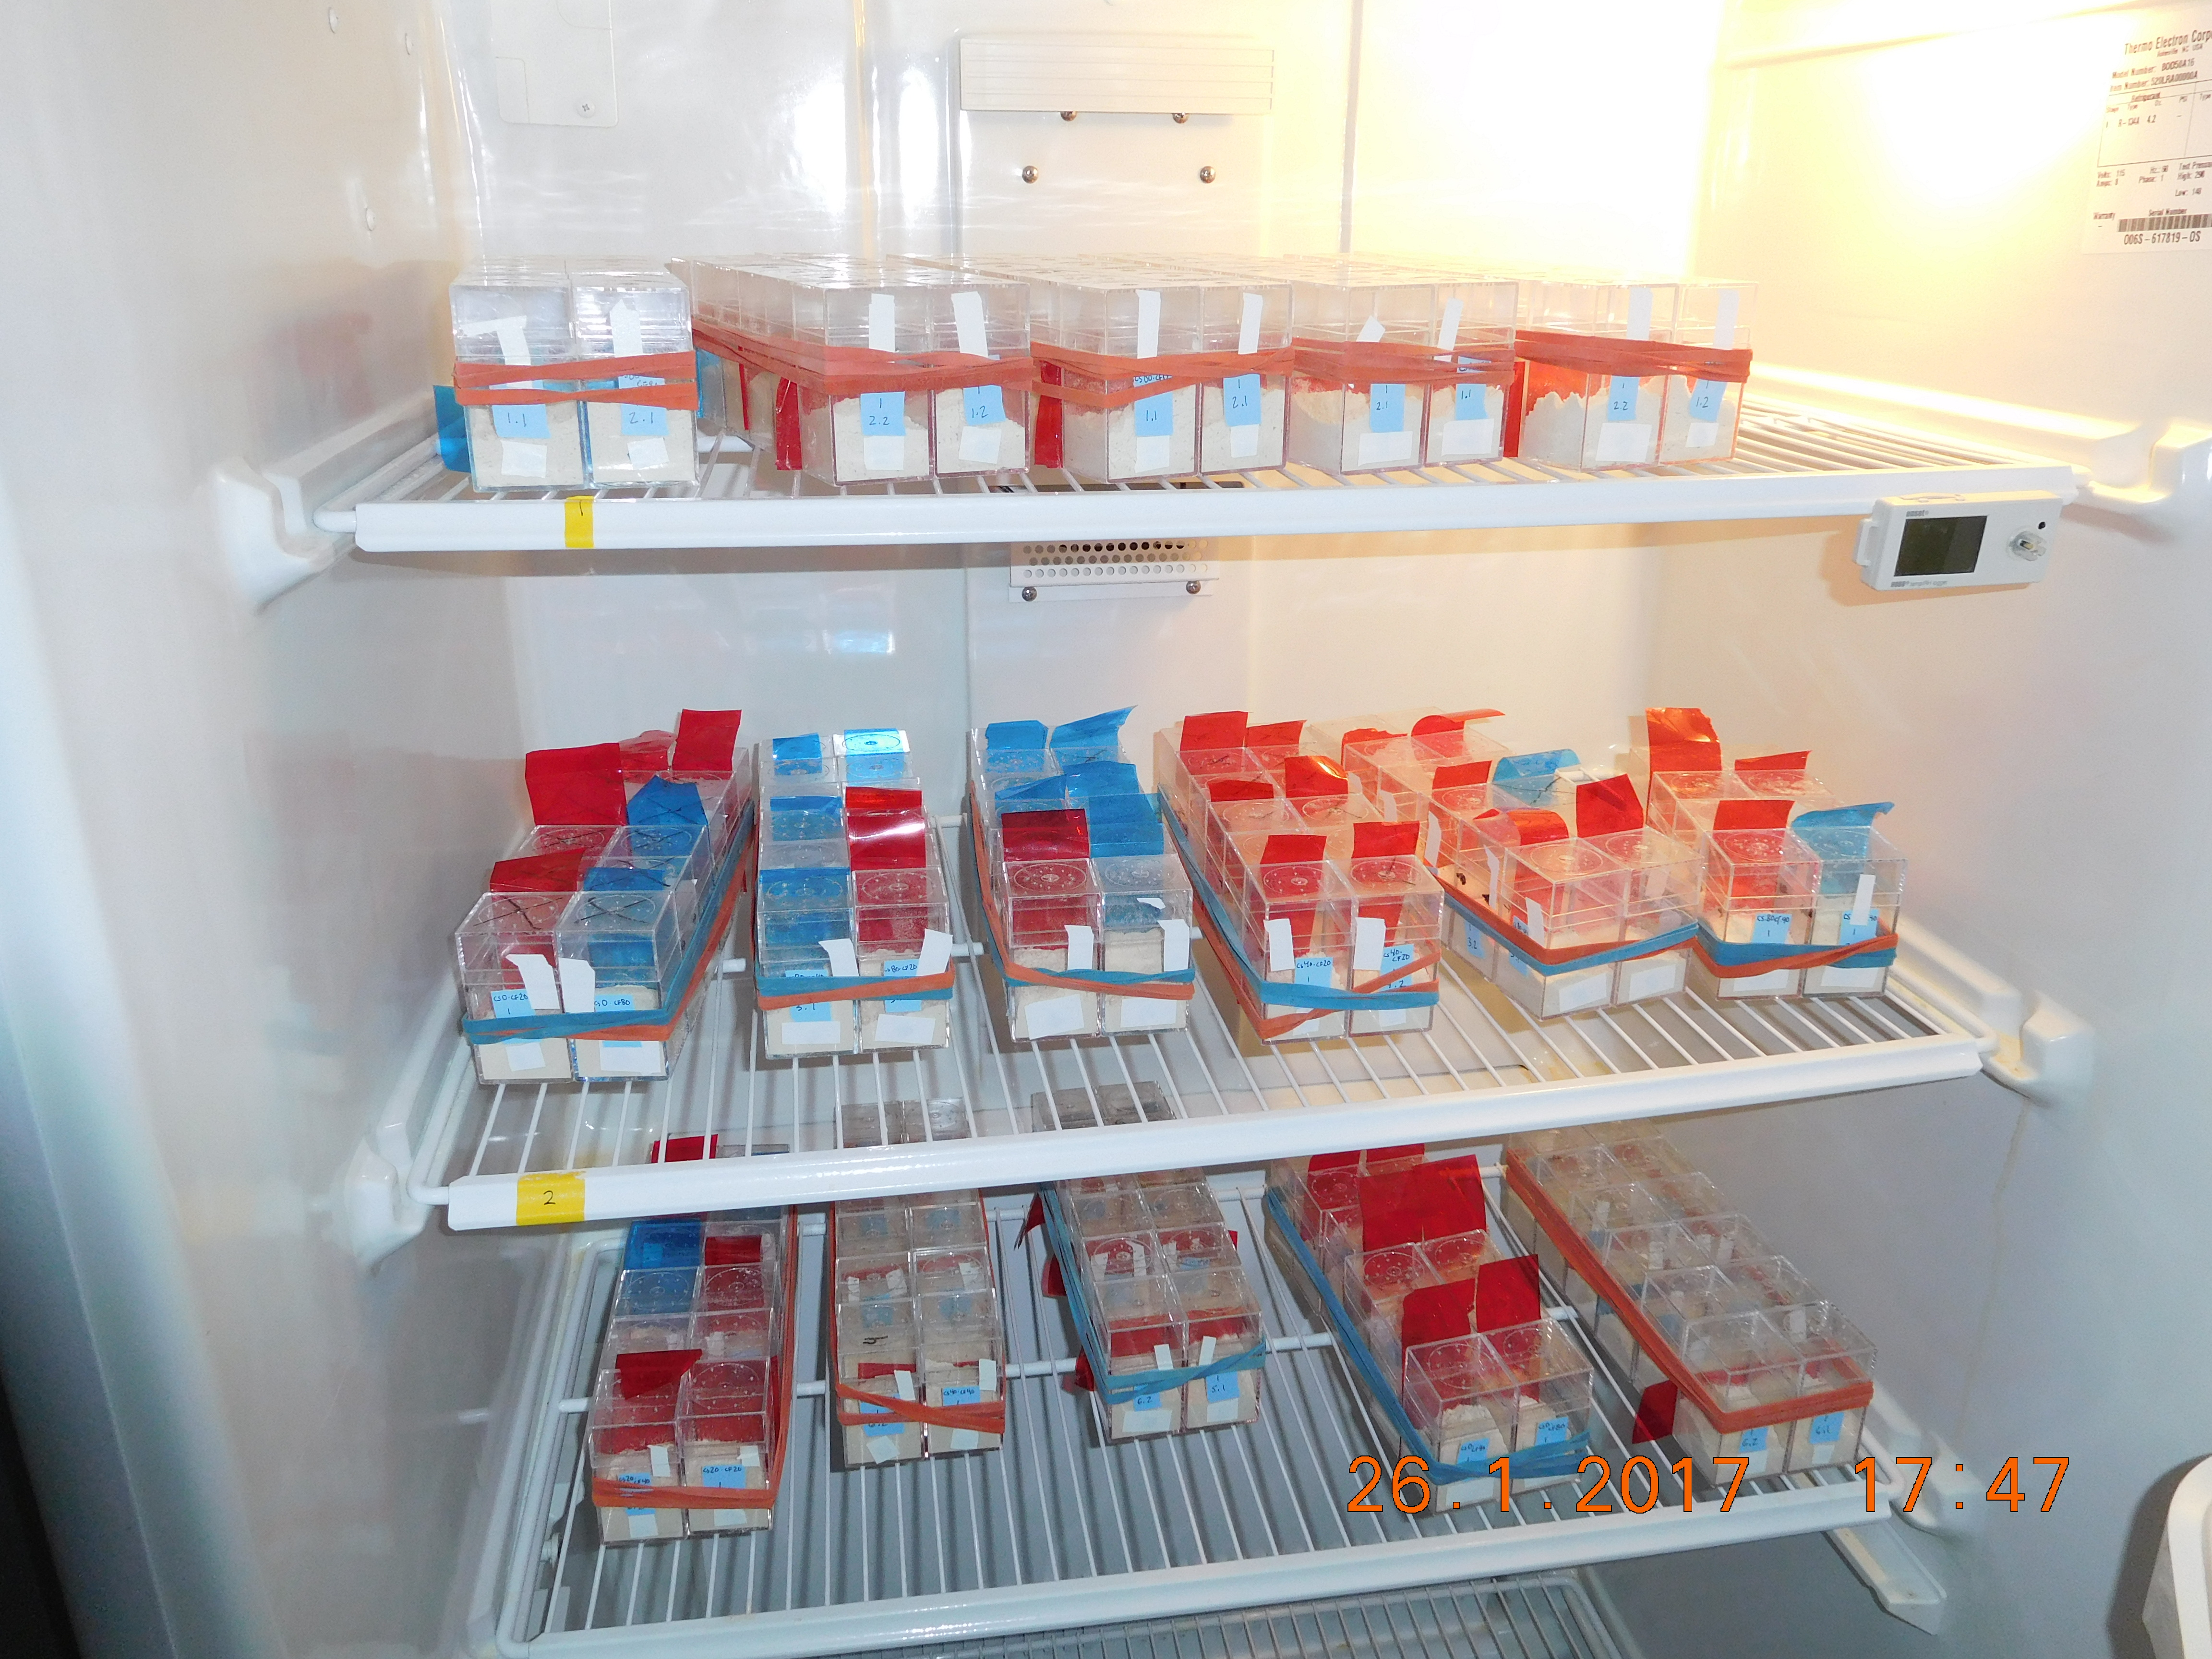
\includegraphics[width=0.75\textwidth]{figs/lab.jpg}
  \end{center}
  \let\thefootnote\relax\footnotetext{Tad Dallas}
\end{frame}








\begin{frame}

	\begin{flushright}
	  \Large \textcolor{boss2}{Ecological modeling} 
	\end{flushright}

%  Generalizing species interactions into systems to equations to understand fundamental processes. This is a very important part of ecology. 

  \begin{center}
    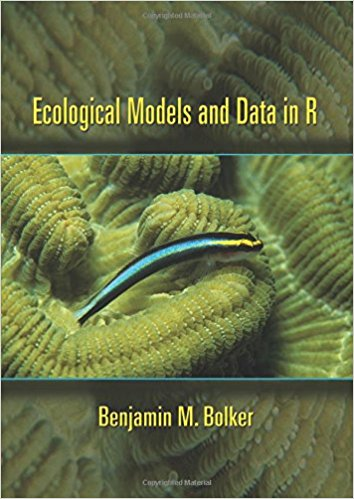
\includegraphics[width=0.4\textwidth]{figs/models.jpg}
  \end{center}
  \let\thefootnote\relax\footnotetext{Ben Bolker}
\end{frame}







\begin{frame}

	\begin{flushright}
	  \Large \textcolor{boss2}{Reading for next week} 
	\end{flushright}

Purugganan, Mary, and Jan Hewitt. "How to read a scientific article." Rice University (2004). \url{https://www.owlnet.rice.edu/~cainproj/courses/HowToReadSciArticle.pdf}

% \url{http://www.imaging.robarts.ca/parraga/How%20To%20Papers/Manuscripts/How%20to%20read%20a%20scientific%20article.pdf}


Ecological Society of America. What does ecology have to do with me? \url{https://www.esa.org/about/what-does-ecology-have-to-do-with-me/}


\end{frame}











\begin{frame}

{\large \textcolor{lsu1}{Contact info}}

  \begin{itemize}
    \item \textcolor{boss1}{Office:} A343 Life Sciences
  \end{itemize}

  \begin{flushright}
    \begin{tabular}{cl}
    
\includegraphics[width=0.75cm]{figs/email.png} & \texttt{tadallas@lsu.edu} \\
    
\includegraphics[width=1.5cm]{figs/octocat.png} & \texttt{taddallas} \\
    
\includegraphics[width=0.75cm]{figs/user.png} & \texttt{taddallas.github.io}\\
   \end{tabular}
  \end{flushright}
\end{frame}













\end{document}
